%%%%%%%%%%%%%%%%%%%%%%%%%%%%%%%%%%%%%%%%%
% Beamer Presentation
% LaTeX Template
% Version 1.0 (10/11/12)
%
% This template has been downloaded from:
% http://www.LaTeXTemplates.com
%
% License:
% CC BY-NC-SA 3.0 (http://creativecommons.org/licenses/by-nc-sa/3.0/)
%
%%%%%%%%%%%%%%%%%%%%%%%%%%%%%%%%%%%%%%%%%

% XXX todo: choose theme from http://deic.uab.es/~iblanes/beamer_gallery/index_by_theme.html
%----------------------------------------------------------------------------------------
%	PACKAGES AND THEMES
%----------------------------------------------------------------------------------------

\documentclass{beamer}

\usepackage[utf8]{inputenc}
\usepackage[T1]{fontenc}
\usepackage{color}

\mode<presentation> {

% The Beamer class comes with a number of default slide themes
% which change the colors and layouts of slides. Below this is a list
% of all the themes, uncomment each in turn to see what they look like.

%\usetheme{default}
%\usetheme{AnnArbor}
%\usetheme{Antibes}
%\usetheme{Bergen}
%\usetheme{Berkeley}
%\usetheme{Berlin}
%\usetheme{Boadilla}
%\usetheme{CambridgeUS}
%\usetheme{Copenhagen}
%\usetheme{Darmstadt}
%\usetheme{Dresden}
%\usetheme{Frankfurt}
%\usetheme{Goettingen}
%\usetheme{Hannover}
%\usetheme{Ilmenau}
%\usetheme{JuanLesPins}
%\usetheme{Luebeck}
\usetheme{Madrid}
%\usetheme{Malmoe}
%\usetheme{Marburg}
%\usetheme{Montpellier}
%\usetheme{PaloAlto}
%\usetheme{Pittsburgh}
%\usetheme{Rochester}
%\usetheme{Singapore}
%\usetheme{Szeged}
%\usetheme{Warsaw}

% As well as themes, the Beamer class has a number of color themes
% for any slide theme. Uncomment each of these in turn to see how it
% changes the colors of your current slide theme.

%\usecolortheme{albatross}
%\usecolortheme{beaver}
%\usecolortheme{beetle}
%\usecolortheme{crane}
%\usecolortheme{dolphin}
%\usecolortheme{dove}
%\usecolortheme{fly}
%\usecolortheme{lily}
%\usecolortheme{orchid}
%\usecolortheme{rose}
%\usecolortheme{seagull}
\usecolortheme{seahorse}
%\usecolortheme{whale}
%\usecolortheme{wolverine}

%\setbeamertemplate{footline} % To remove the footer line in all slides uncomment this line
%\setbeamertemplate{footline}[page number] % To replace the footer line in all slides with a simple slide count uncomment this line

%\setbeamertemplate{navigation symbols}{} % To remove the navigation symbols from the bottom of all slides uncomment this line
}

\usepackage{graphicx} % Allows including images
\usepackage{booktabs} % Allows the use of \toprule, \midrule and \bottomrule in tables

%----------------------------------------------------------------------------------------
%	TITLE PAGE
%----------------------------------------------------------------------------------------

\title[User Namespaces]{What's CGManager doing and why is it still relevant} % The short title appears at the bottom of every slide, the full title is only on the title page

\author{Serge Hallyn} % Your name
\institute[Canonical] % Your institution as it will appear on the bottom of every slide, may be shorthand to save space
{
Canonical, Inc \\ % Your institution for the title page
\medskip
\textit{serge.hallyn@ubuntu.com} % Your email address
}
\date{\today} % Date, can be changed to a custom date

\begin{document}

\begin{frame}
\titlepage % Print the title page as the first slide
\end{frame}

\begin{frame}
\frametitle{Overview}

\textbf{Agenda:}
\begin{itemize}
\item CGroup intro
\item Containers
\item Requirements from lxc
\item Cgmanager details
% \item Demonstration
\item Future and alternatives
\end{itemize}
\end{frame}

\begin{frame}
\frametitle{About me}
\begin{itemize}
\item Ubuntu server team member
\item Started with linux kernel in 1998
\item Working with containers since ``vpid'' and ``nsproxy'' in 2006
\item Upsteam lxc maintainer
\item Author of cgmanager
\end{itemize}
\end{frame}


\begin{frame}
\frametitle{Cgroups}
\begin{itemize}
\item Introduced in 2007 as "task containers"
\item Group tasks
\item Track and Limit Resource Usage
\item Memory, Cpuset, Devices, BlockIO, etc. \\
Grouped together or separately.
\item Administered through filesystem interface \\ 
\vspace{0.2in}
{\tt \small mkdir -p /freezer \\
mount -t cgroup -o freezer freezer /freezer \\
mkdir /freezer/group1 \\
sleep 200 \& echo \$! > /freezer/group1/tasks \\
echo FROZEN > /freezer/group1/freezer.state}
\end{itemize}
\end{frame}

\begin{frame}
\frametitle{Containers}
\begin{itemize}
\item OS level virtualization
\item Userspace fiction
\item Uses many kernel features to emulate VM
\item Uses cgroups for tracking and resource control
\item Can be used without privilege
\item Can be nested
\end{itemize}
\end{frame}

\begin{frame}
\frametitle{Why cgmanager}
\textbf{Safe, unprivileged, nested containers}
\begin{itemize}
\item Delegating cgfs to users discouraged
\item Full delegation not possible with cgroupfs (devices)
\item Avoid need to grant safe access to cgroupfs
\item Prevent escaping to parent cgroups even if root
\item Potential for intelligence
\end{itemize}
\textbf{Simplify nesting}
\begin{itemize}
\item Task in {\tt /lxc/c1/user.slice/user-1000.slice/session-c1.scope}
\item Starts container c2:
	\begin{itemize}
	\item As root, in {\tt /lxc/c1/lxc/c2}
	\item Unprivileged, in {\tt/lxc/c1/user.slice/user-1000.slice/session-c1.scope/c2}
	\item Never as {\tt /lxc/c2}
	\end{itemize}
\end{itemize}
\end{frame}

\begin{frame}
\frametitle{Why cgmanager}
\textbf{Simplify cgroup management code}
\begin{itemize}
\item {\tt /proc/self/cgroup} shows full paths
\item Many hierarchy co-mounting possibilities
  \begin{itemize}
  \item All subsystems co-mounted
  \item All separately mounted
  \item Some co-mounted
  \item Cgroup membership may be very different per hierarchy
  \end{itemize}
\item Many cgroupfs mounting possibilities
  \begin{itemize}
  \item No mount at all
  \item Full mount of cgroup fs under /sys/fs/cgroup/subsys
  \item Bind-mount of {\tt /lxc/c1} under /sys/fs/cgroup/subsys
  \item Empty dirs up to {\tt /sys/fs/cgroup/subsys/lxc/c1} bind-mount
  \end{itemize}
\end{itemize}
\end{frame}

\begin{frame}
\frametitle{CGManager}
\begin{itemize}
\item Proposed idea November 25 2013
\item Used by lxc, upstart, systemd-shim, and libvirt
\end{itemize}
\end{frame}

\begin{frame}
\frametitle{Cgmanager Design}

\begin{itemize}
\item One daemon per host
\item Requests placed over dbus
\begin{itemize}
\item {\tt /sys/fs/cgroup/cgmanager/sock}
\item Cannot send pid, uid, gid across namespaces using dbus
\end{itemize}
\end{itemize}
\end{frame}

\begin{frame}
\frametitle{Limits of DBus Request}
% 128 x 96 is default slide
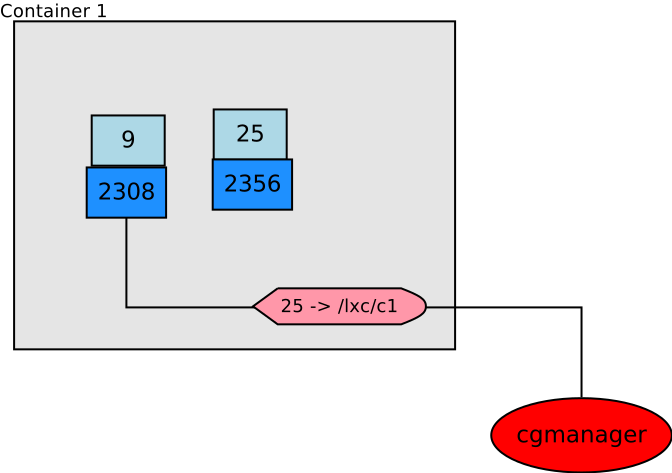
\includegraphics[width=110mm]{pidmessage.png}
\end{frame}

\begin{frame}
\frametitle{Cgmanager Design}
\begin{itemize}
\item {\color{blue}One daemon per host}
\item {\color{blue}Requests placed over dbus}
	\begin{itemize}
	\item {\color{blue}Cannot send pid, uid, gid across namespaces using dbus}
		\begin{itemize}
		\item setns requires newer kernel
		\item setns(CLONE\_NEWUSER) drops global capabilities
		\end{itemize}
	\item Send pids and uids as SCM credentials
	\end{itemize}

\end{itemize}
\end{frame}

\begin{frame}
\frametitle{SCM-Enhanced DBus Request}
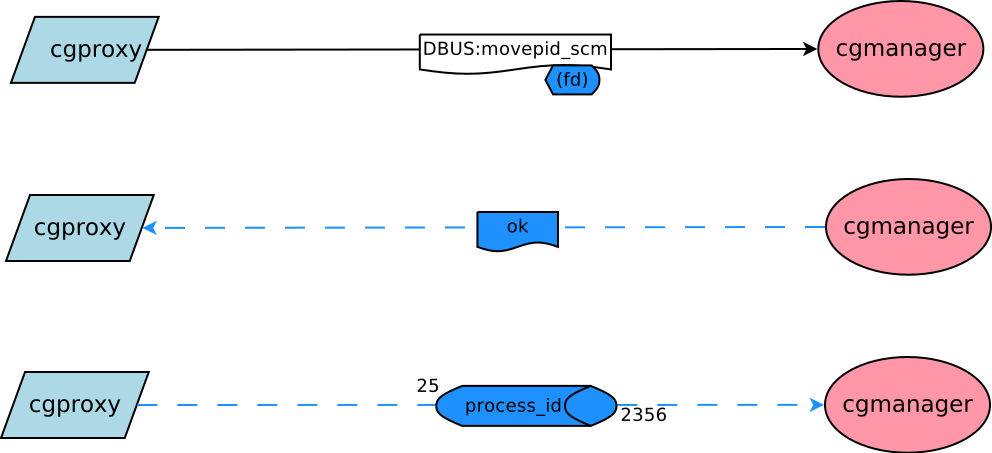
\includegraphics[width=110mm]{scm.png}
\end{frame}

\begin{frame}
\frametitle{Cgmanager Design}
\begin{itemize}
\item {\color{blue}One daemon per host}
\item {\color{blue}Requests placed over dbus}
	\begin{itemize}
	\item {\color{blue}Cannot send pid, uid, gid across namespaces using dbus}
		\begin{itemize}
		\item {\color{blue}setns requires newer kernel}
		\item {\color{blue}setns(CLONE\_NEWUSER) drops global capabilities}
		\end{itemize}
	\item {\color{blue}Send pids and uids as SCM credentials}
	\end{itemize}
\item One proxy per container
\item Request can be sent as plain dbus to proxy in same ns
\item All proxies connect to the host's cgmanager
\item ``README'' details the security guarantees
\end{itemize}
\end{frame}

\begin{frame}
\frametitle{Proxy architecture}
\includegraphics[width=110mm]{proxies.png}
\end{frame}

\begin{frame}
\frametitle{Sockets}
\begin{itemize}
\item Cgmanager listens on {\tt /sys/fs/cgroup/cgmanager/sock}
\item Lxc bind-mounts that directory into containers
\item Cgproxy moves {\tt /sys/fs/cgroup/cgmanager} $\rightarrow$
{\tt /sys/fs/cgroup/cgmanager.lower}
\item Cgproxy listens on {\tt /sys/fs/cgroup/cgmanager/sock}
\item If {\tt /sys/fs/cgroup/cgmanager.lower} exists, lxc moves that into container
\end{itemize}
\end{frame}

\begin{frame}
\frametitle{CGroup Namespace}
\begin{itemize}
\item DBus requests are relative to your current cgroup \\
	Create(new) $\rightarrow$ Create(current\_cgroup . new)
\item {\tt /lxc/c1/user.slice/user-1000.slice/session-c1.scope} $\rightarrow$
{\tt /lxc/c1/user.slice/user-1000.slice/session-c1.scope/new}
\item But root wants to create {\tt /lxc/c1/lxc/c2}
\item But should never be able reference {\tt /lxc/c3}
\item ``Escape'' supported to your proxy's cgroup for:
	\begin{itemize}
	\item MovePidAbs: for root in cgmanager's pid namespace
	\item MovePidAbsScm: Relative to proxy's cgroup
	\item GetPidCgroupAbs: Relative to proxy's cgroup
	\end{itemize}
\end{itemize}
\end{frame}

\begin{frame}
\frametitle{DBus methods}
\begin{itemize}
\item Ping, ApiVersion
\item GetPidCgroup, MovePid, Create, Chmod
\item Chown(X, Uid, Gid):
	\begin{itemize}
	\item Requires w$\rightarrow$ X, privilege over Uid, Gid
	\item Chowns X, X/tasks, X/cgroup.procs, but not other X/*
	\item Uid may create X/* and move tasks, but not change limits
	\end{itemize}
\item GetValue, SetValue
	\begin{itemize}
	\item Limits specified using cgroup filenames
	\item Lxc has exported these since 2008
	\item New API would be temporary
	\item Minimize churn for lxc
	\end{itemize}
\item GetTasks, GetTasksRecursive, ListChildren
\item Remove, RemoveOnEmpty, Prune
\item ListControllers, ListKeys
\end{itemize}
\end{frame}

\begin{frame}
\frametitle{Future: Possibilities:}
\textbf{Possible Alternatives}

\begin{itemize}
\item Enhance cgfs
	\begin{itemize}
	\item Fake root (cgroup namespaces, Aditya Kali@google, July 2014)
	\item Full delegation
	\end{itemize}

\item Enhance systemd slices
	\begin{itemize}
	\item Allow users to specify sub-slices
	\item Wider resource support (net\_cls, etc)
	\item Support delegation to user namespaces \\
	Uid 100000 may act on uid 100005
	\end{itemize}

\item Continue with CGManager
	\begin{itemize}
	\item Get/SetValue (key/value) API (Abstract away cgfs filenames?)
	\item Support new remove-on-empty mechanism
	\item Keep state (hotplug, etc)
	\item Integrate with systemd
	\end{itemize}
\end{itemize}
\end{frame}

\begin{frame}
\frametitle{Comments, Questions}
\textbf{ serge.hallyn@ubuntu.com }
\end{frame}


\end{document}
